\documentclass[12pt]{article}

% packages

%\usepackage{times} % alt: cmbright
\usepackage[top=1in, bottom=1in, left=1in, right=1in]{geometry}
\usepackage{natbib}
\usepackage{amsmath}
\usepackage{amssymb}
\usepackage{latexsym}
\usepackage{sectsty}
\usepackage{amsfonts}
\usepackage{epsfig}
\usepackage{url}
\usepackage{microtype}
\usepackage{fixmath}
\usepackage{hyperref}
\usepackage{amsthm}
\usepackage{subfigure}
\usepackage{float}
\usepackage{hyperref}

\newtheorem{lem}{Lemma}
\newtheorem{defn}{Assumption}
\newtheorem{propty}{Property}
\newtheorem{thm}{Theorem}

% references

\newcommand{\mysec}[1]{Section~\ref{sec:#1}}
\newcommand{\myapp}[1]{Appendix~\ref{app:#1}}
\newcommand{\myeq}[1]{Equation~\ref{eq:#1}}
\newcommand{\myeqp}[1]{Eq.~\ref{eq:#1}}
\newcommand{\mychap}[1]{Chapter~\ref{chap:#1}}
\newcommand{\myfig}[1]{Figure~\ref{fig:#1}}

% math conveniences

\newcommand{\g}{\,\vert\,}
\newcommand{\E}{\textrm{E}}
\newcommand{\vct}[1]{\textbf{#1}}
\newcommand{\realline}{\mathbb{R}}
\newcommand{\indpt}{\protect\mathpalette{\protect\independenT}{\perp}}
\def\independenT#1#2{\mathrel{\rlap{$#1#2$}\mkern2mu{#1#2}}}
\newcommand{\h}[1]{\textrm{H}\left( #1 \right)}
\newcommand{\half}{\frac{1}{2}}
\newcommand{\new}{\textrm{new}}

\newcommand{\mult}{\textrm{Mult}}
\newcommand{\dir}{\textrm{Dir}}
\newcommand{\discrete}{\textrm{Discrete}}
\newcommand{\Bern}{\textrm{Bern}}
\newcommand{\DP}{\textrm{DP}}
\newcommand{\GP}{\textrm{GP}}
\newcommand{\Bet}{\textrm{Beta}}

% paragraph spacing

\setlength{\parindent}{0pt}
\setlength{\parskip}{2ex plus 0.5ex minus 0.2ex}

\allsectionsfont{\sffamily\mdseries}
\paragraphfont{\sffamily\bfseries}

\usepackage{algorithm}
\usepackage{algorithmic}
\renewcommand{\algorithmicrequire}{\textbf{Input:}}
\renewcommand{\algorithmicensure}{\textbf{Output:}}


\begin{document}

\title{\textsf{Approximating Multi-Objective Optimization using Particle Swarm}}
%\author{\textsf{Daqing Yi}}
\date{\textsf{Brigham Young University}}

\maketitle

\section{Multi-Objective Optimization}

Multi-objective optimization is a class of problems with solutions that can be evaluated along two or more incomparable or conflicting objectives.

Without loss of generality, we focus only on minimization objective in this paper. 
Because any minimum objective can be converted into a maximum objective by adding a negative operator, and vice verse. 

\begin{mydef}[\textbf{Multi-Objective Optimization}]
\label{def:multi_opt}
Find the vector $ \vec{x}^{*} \in S $ which will satisfy the $ m $ inequality constraints
\begin{equation}
\label{eq:mo_ineq_constraint}
g_{i}(\vec{x}) \geq 0, i = 1, 2, \cdots , m, 
\end{equation}
the $ p $ equality constraints
\begin{equation}
\label{eq:mo_eq_constraint}
h_{i}(\vec{x}) = 0, i = 1, 2, \cdots , p, 
\end{equation}
and will optimize the vector function
\begin{equation}
\label{eq:mo_obj}
\min_{ S } \vec{f}(\vec{x}) = \min_{ S } \left[ f_{1}(\vec{x}), f_{2}(\vec{x}) \cdots f_{k}(\vec{x}) \right]^{T},
\end{equation}
where $ \vec{x} $ is the vector of decision variables.
\end{mydef}

Here we would like to emphasize that there exists two spaces in a multi-objective optimization problem, which are
\emph{solution space} $ S \subset \mathbb{R}^{n}  $ and \emph{evaluation space} $ Z \subset \mathbb{R}^{k} $.
$ \vec{f}() $ maps a position $ x \in S $ to a position $ z \in Z $.

Due to the incomparability and conflict between objectives, there is usually no solution that satisfies all the objectives.
We import \emph{dominance} to describe a relationship between any two solutions.

\begin{mydef}[\textbf{Dominance}]
\label{def:dominance}
$ \vec{x} \in S $ dominates $ \vec{x'} \in S $, if 
\begin{equation}
\label{eq:def_dominance}
\forall i \in \{ 1, 2, \cdots k \}, f_{i}(\vec{x}) \leq f_{i}(\vec{x'}).
\end{equation}
We write it as $ \vec{x} \preceq \vec{x'} $.

$ \vec{x}  $ is non-dominant, if 
\begin{equation}
\label{eq:def_nondominant}
\nexists \vec{x'} \in S \land \vec{x'} \neq \vec{x}, \vec{x'} \preceq \vec{x}.
\end{equation}
\end{mydef}

A set of all the non-dominant solutions is called a \emph{Pareto set}.
\begin{mydef}[\textbf{Pareto set}]
\label{def:pareto_opt_set}
For a given multi-objective optimization problem $ \vec{f}() $, the \emph{Pareto optimal set} $ P^{*}_{S} \subset S $ is defined as
\begin{equation}
\label{eq:pa_opt_set}
P^{*}_{S} := \{ \vec{x} \in S \mid \nexists \vec{x}' \in S, \vec{x'} \preceq  \vec{x} \}.
\end{equation}

\end{mydef}

\emph{Pareto set} defines \emph{Pareto optimal} for the multi-objective optimization problems.
In the evaluation space $ Z $, we have a \emph{Pareto front} mapped from \emph{Pareto set} by $ \vec{f}() $.

\begin{mydef}[\textbf{Pareto Front}]
\label{def:pareto_front}
For a given multi-objective optimization problem $ \vec{f}() $ and Pareto optimal set $ P^{*}_{S} \subset S $, the \emph{Pareto front} $ P^{*}_{Z} \subset Z $ is defined as
\begin{equation}
\label{eq:pa_front}
P^{*}_{Z} := \{ \vec{z} = \vec{f}(\vec{x}) \mid \vec{x} \in P^{*}_{S} \}.
\end{equation}
\end{mydef}

\begin{figure} 
  \centering 
  \subfigure[Solution space]{ 
    \label{fig:sol_space} %% label for first subfigure 
    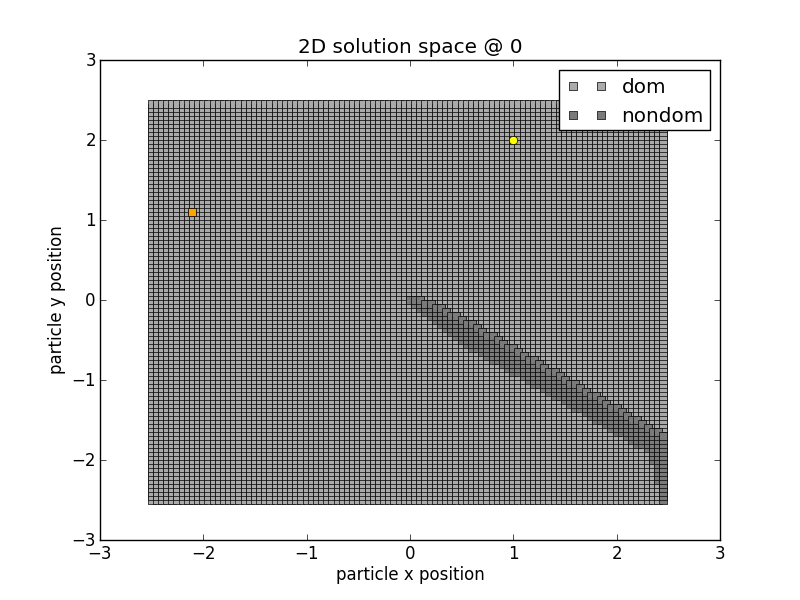
\includegraphics[width=0.45\textwidth]{./images/solution_space.png}} 
  %\hspace{1in} 
  \subfigure[Evaluation space]{ 
    \label{fig:eval_space} %% label for second subfigure 
    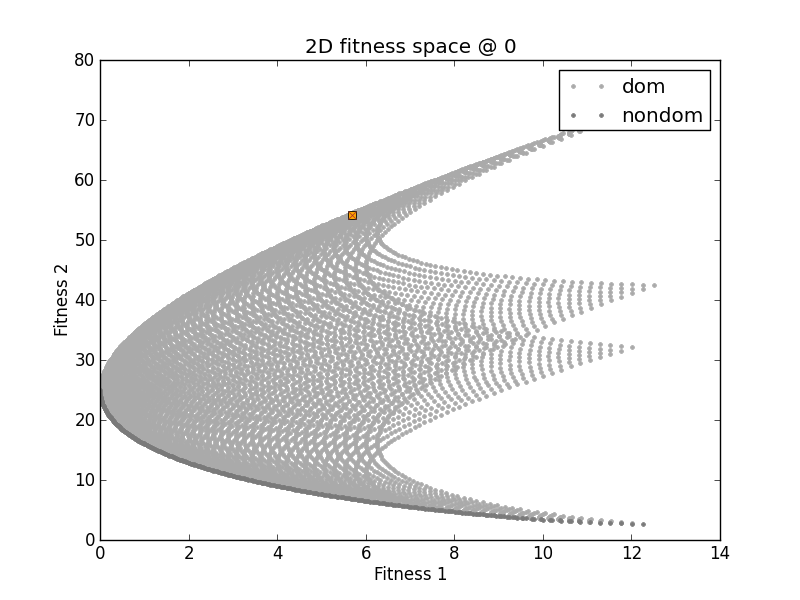
\includegraphics[width=0.45\textwidth]{./images/evaluation_space.png}}      
  \caption{Mapping between solution space and evaluation space.}
  \label{fig:space_mapping} %% label for entire figure 
\end{figure}

Due to how \emph{Pareto optimal} is defined, there is no straightforward way to solve like that in a conventional single-objective optimization problem.
Evolutionary algorithms are popular approaches to the multi-objective optimization problems. 

In this paper, we are interested with how to use \emph{Particle swarm optimization} to solve the multi-objective optimization problems.

\section{Particle Swarm Optimization}

\begin{mydef}[\textbf{Particle Swarm Optimization}]
\label{def:pso}

Let $ X $ be a set of particles.  
A \emph{particle} is a data structure that maintains current position $ \vec{x}_{i} $ and current velocity  $ \vec{v}_{i} $.
Denote $ \vec{x}^{P}_{i} $ for ``personal best'', which is the most fit position remembered of a particle. 
Denote $ \vec{x}^{G}_{i} $ for ``global best'', which is most fit $ \vec{x}^{P}_{i} $ among all particles. 
The algorithm runs as below:
\begin{enumerate}
\item Scattering particles $ \vec{x}_{i}(0) $ in decision space stochastically
\item Each particle update its location over time \\
\begin{equation}
\label{eq:up_vel}
\begin{aligned}
\vec{v}_{i}(t) & = \chi [ \vec{v}_{i}(t-1) + \phi^{P} \vec{u}^{P}_{i}(t-1) \otimes (\vec{x}^{P}_{i}(t-1) - \vec{x}_{i}(t-1)) \\
& + \phi^{G} \vec{u}^{G}_{i}(t-1) \otimes (\vec{x}^{G}_{i}(t-1) - \vec{x}_{i}(t-1)) ],
\end{aligned}
\end{equation}
\begin{equation}
\label{eq:up_pos}
\vec{x}_{i}(t) = \vec{x}_{i}(t-1) + \vec{v}_{i}(t),
\end{equation}
in which each element of $ \vec{u}^{P}_{i}(t-1) $ and $ \vec{u}^{G}_{i}(t-1) $ is independently sampled from uniform distribution $ [0, 1] $.
\end{enumerate}
\end{mydef}

We intends to use $ \vec{f}(X) $, which is the positions of the particle set $ X $ in the evaluation space, to approximate the Pareto front $ P^{*}_{S} $.
In order to measure how the approximation is, we look at two factors:
\begin{itemize}
\item how the particles moves close into the Pareto front;
\item how the diversity of the particles is.
\end{itemize}

\subsection{Set distance measurement}

We import \emph{Hausdorff distance} [\cite{schutze2012using}] to measure the distance between a set $ A $ and a set $ B $.
\begin{mydef}[\textbf{Hausdorff Distance}]
\label{def:haus_dist}
Let $ u, v \in \mathbb{R}^{n} $, and $ || \cdot || $ be a vector norm.
The Hausdorff distance $ d_{H} $ is defined as:
\begin{itemize}
\item $ dist(u, B) = \inf_{v \in B} || u - v ||  $;
\item $ dist(A, B) = \sup_{u \in A} dist(u, B) $;
\item $ d_{H} (A, B) = \max (dist(A,B), dist(B,A)) $.
\end{itemize}
\end{mydef}

\begin{figure}
\centering
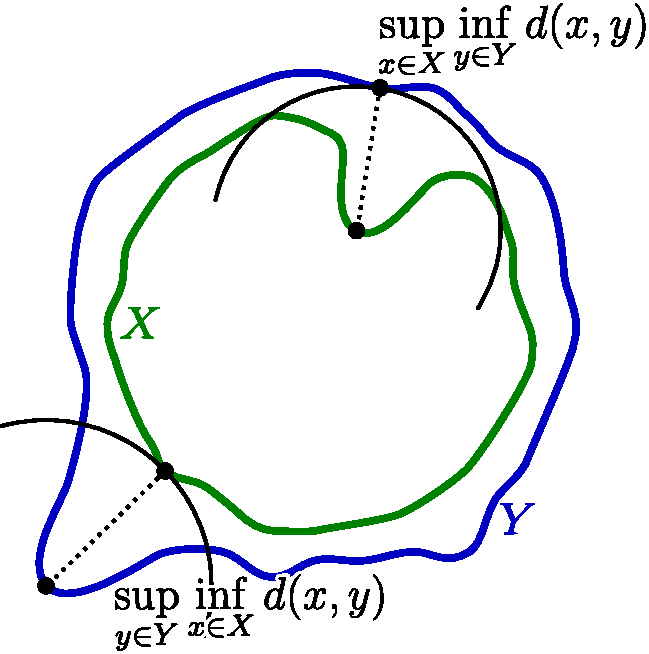
\includegraphics[width=0.3\linewidth]{./images/hausdorff_distance}
\caption{Hausdorff distance.}
\label{fig:hausdorff_distance}
\end{figure}

Figure \ref{fig:hausdorff_distance} gives an exmaple on how the Hausdorff distance is defined.

If we assume that $ || y - x || = || x - y || $, we can have Hausdorff distance as
\begin{equation}
\label{eq:simp_haus_dist}
d_{H} (A, B) = \sup_{u \in A} \left( \inf_{v \in B} || u - v || \right).
\end{equation} 

We notice that when $ A \subset B $, $ d_{H}(A, B) = 0 $.
In our case, it means that all the particles moves into the Pareto set.

When all the particles are in the Pareto set, we turn to look at the diversity.

\subsection{Diversity measurement}

There are several ways of measuring diversity proposed in research works. 

\cite{risco2008optimization} proposed \emph{spacing} to measure diversity, which is 
\begin{equation}
\begin{aligned}
S & = \sqrt{\frac{1}{n-1}\sum_{i=1}^{n}(\bar{d}-d_{i})^{2}}, \\
d_{i} & = \min_{j} || \vec{f}(\vec{x_{i}}) - \vec{f}(\vec{x_{j}}) ||, i,j \in \{ 1, \cdots , n \}, \\
\bar{d} & = \frac{1}{n} \sum_{i=1}^{n} d_{i}.
\end{aligned}
\end{equation}

\cite{silva2013multi} proposed a \emph{diversity factor} for each single particle to measure the diversity, which is:
\begin{equation}
\begin{aligned}
d_{i} & = \frac{1}{n-1} \sum_{j=1, j \neq i}^{n} || \vec{f}(\vec{x_{i}}) - \vec{f}(\vec{x_{j}}) ||, \\
DF_{i} & = \frac{ d_{i} - d_{min} }{ d_{max} - d_{min} }
\end{aligned}
\end{equation}

\cite{coello2005solving} uses a \emph{Inverted generational distance}, which is:
\begin{equation}
\begin{aligned}
GD & = \frac{\sqrt{\sum_{i=1}^{n} d_{i}^{2} }}{n} \\
d_{i} & = \min_{j} || \vec{f}(\vec{x_{j}}) - \vec{f}(\vec{x_{i}}) ||
\end{aligned}
\end{equation}

\cite{olorunda2008measuring} use a \emph{normalized average distance around the swarm center} to measure the diversity, which is:
\begin{equation}
\begin{aligned}
D^{N} & = \frac{1}{n} \sum_{i=1}^{n} D^{N}_{i} \\
D^{N}_{i} & = \frac{1}{n \times D} \sum_{j=1}^{n} || \vec{f}( \vec{x_{i}} ) - \vec{f}( \vec{x_{j}} ) || \\
D & = \max_{i \neq j} || \vec{f}( \vec{x_{i}} ) - \vec{f}( \vec{x_{j}} ) ||
\end{aligned}
\end{equation}

\cite{pires2013entropy} divides the solution space into $ N $ cells, use $ n_{i} $ to denote the number of particles in cell $ i $. Thus an entropy value can be obtained by
\begin{equation}
\begin{aligned}
H = \sum_{1}^{N} \frac{n_{i}}{N} \log{ \frac{n_{i}}{N} }.
\end{aligned}
\end{equation}

\begin{hyp}
\label{hyp:pareto_convex}
Pareto set is convex.
\end{hyp}

Here we are interested that each particle can maximize its distance to the nearest other particle in the evaluation space, which is
\begin{equation}
\label{eq:diversity_dist}
\sup_{v \in X \setminus x} || \vec{f}(x) - \vec{f}(v) ||.
\end{equation}


Formally, we define two metrics to mesaure how $ \vec{f}(X) $ approximate the Pareto front $ P^{*}_{Z} $. They have priority by order.
\begin{itemize}
\item minimizing $ \sup_{x \in X}  \left( \inf_{z \in P^{*}_{Z} } || \vec{f}(x) - z  || \right) $,
\item maximizing $ \sum_{u \in X} \left( \sup_{v \in X \setminus u} || \vec{f}(u) - \vec{f}(v) || \right) $.
\end{itemize}

For each single particle, the equivalent metrics can be 
\begin{itemize}
\item minimizing $  \min_{z \in P^{*}_{Z} } || \vec{f}(x) - z  ||  $,
\item maximizing $ \max_{v \in X \setminus u} || \vec{f}(u) - \vec{f}(v) ||  $.
\end{itemize}

With the metrics defined, we are interested with how to design the PSO algorithm to make the expected behaviors of the particles.

\section{Particle Swarm}

\cite{coello2002mopso} proposed to use a randomly choosing global best or personal best from archives to make particles diverse. 
Rather than randomly selecting, \cite{mostaghim2003strategies} calculate a sigma value for selecting a personal best from the archives for a particle.
In a similar idea, \cite{raquel2005effective} uses a crowding distance in global best selection to maintain the diversity.

\cite{alvarez2005mopso} introduced Pareto dominance to global best selection.
\cite{balling2003maximin} firstly proposed a maximin fitness function applied to multi-objective optimization. 
Based on that, \cite{li2004better} import this fitness to the PSO algortihm.

We modify a canonical PSO algoritm presented in Definition \ref{def:pso} for the multi-objective optimization problem on two terms, which are \emph{fitness function} and \emph{personal best}.

By comparing $ \vec{f}(x) $, we can categorize the particles into two types, which are \emph{non-dominated} and \emph{dominated}.
We are use the subset of all the non-dominated particle as the estimation of the Pareto set, which is written as $ \hat{P^{*}_{S}} $.

\subsection{Fitness function}

By comparing with all non-dominated particles, we define the maximum fitness function similar with that in [\cite{li2004better}].
For a particle $ x \in X $,
\begin{equation}
\label{eq:maximin_fitness}
fitness(x) = \max_{y \in \hat{P^{*}_{S}} \land y \neq x} \left( \min_{i=1, \cdots , k} [ f_{i}(x) - f_{i}(y) ] \right).
\end{equation}

We take case analysis on $ x $, which are $ x \notin \hat{P^{*}_{S}} $ and $ x \in \hat{P^{*}_{S}} $.
It is noticeable that when $ x \notin \hat{P^{*}_{S}} $, it means that $ \exists y \in X, y \preceq x $. Thus $ x \not \in P^{*}_{S} $.
However, when $ x \in \hat{P^{*}_{S}} $, it is still possible that $ x $ is dominated by some $ y \in S $. Thus $ x $ can either be $ \in P^{*}_{S} $ or $ \notin \in P^{*}_{S} $.


\begin{itemize}

\item $ x \notin \hat{P^{*}_{S}} $ \\
We can see that
\begin{equation}
x \notin \hat{P^{*}_{S}} \Rightarrow  \forall y \in X \setminus x, \min_{i=1, \cdots , k} [ f_{i}(x) - f_{i}(y) ] > 0,
\end{equation}
which means
\begin{equation}
x \notin \hat{P^{*}_{S}} \Rightarrow fitness(x) > 0.
\end{equation}

Minizing $ fitness(x) $ will minimize $  \min_{z \in P^{*}_{Z} } || \vec{f}(x) - z  ||  $

\item $ x \in \hat{P^{*}_{S}} $ \\
We can see that
\begin{equation}
x \in \hat{P^{*}_{S}} \Rightarrow \forall y \in X \setminus x, \min_{i=1, \cdots , k} [ f_{i}(x) - f_{i}(y) ] \leq 0,
\end{equation}
which means
\begin{equation}
x \in \hat{P^{*}_{S}} \Rightarrow fitness(x) \leq 0.
\end{equation}

If $ x \in P^{*}_{S} $, it means $  \min_{z \in P^{*}_{Z} } || \vec{f}(x) - z  ||  = 0 $, which is minized.
Because $ fitness(x) \leq 0 $, minimizing $ fitness $ will actually increase $ \max_{v \in X \setminus u} || \vec{f}(u) - \vec{f}(v) ||  $.

\end{itemize}

\subsection{Personal Best}

Assume that the swarm has good knowledge or estimation on where the Pareto front locates.
By how we design the fitness function and the equations of the canonical PSO algortim, we can consider that each particle has two forces in moving, which are
\begin{itemize}
\item from ``global best'';
the force $ \vec{x}^{G}_{i}(t-1) - \vec{x}_{i}(t-1) $ pulls the particle towards the Pareto front;

\item from ``personal best'';
the force $ \vec{x}^{P}_{i}(t-1) - \vec{x}_{i}(t-1)) $ has two stages:
\begin{itemize}
\item when $ x \notin P^{*}_{S} $, it pulls the particle towards the Pareto front;
\item when  $ x \in P^{*}_{S} $, it pushes the particle for diversity.
\end{itemize}

\end{itemize}

\cite{branke2006selecting} reivewed the function of personal best selection in multi-objective optimization problems. 
They analyzed several ways of personal best selection to illustrate its function on convergence and diversity.
The person best can be uniformly randomly sampled from known non-dominated solutions, which attracts the particle to some position in the Pareto front.

\begin{figure} 
  \centering 
  \subfigure[Solution space]{ 
    \label{fig:sol_space_perfect} %% label for first subfigure 
    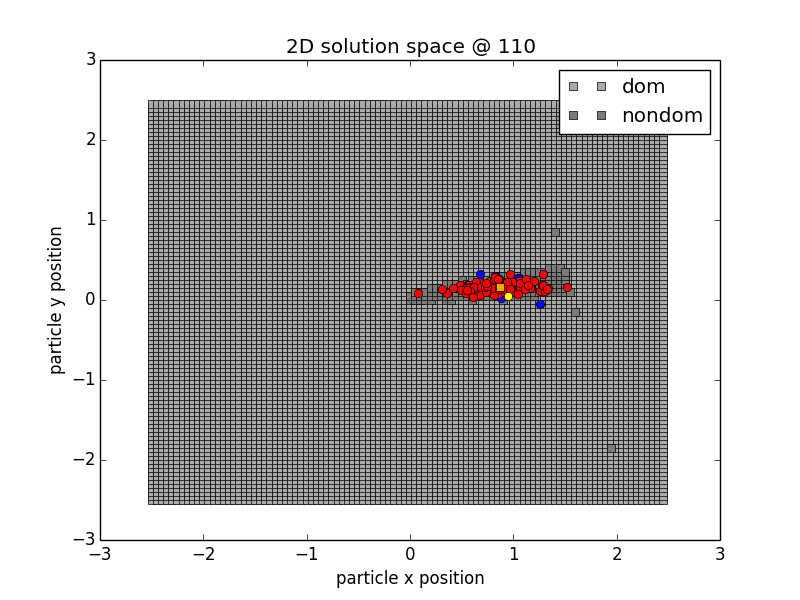
\includegraphics[width=0.45\textwidth]{./images/solution_space_perfect_knowledge.png}} 
  %\hspace{1in} 
  \subfigure[Evaluation space]{ 
    \label{fig:eval_space_perfect} %% label for second subfigure 
    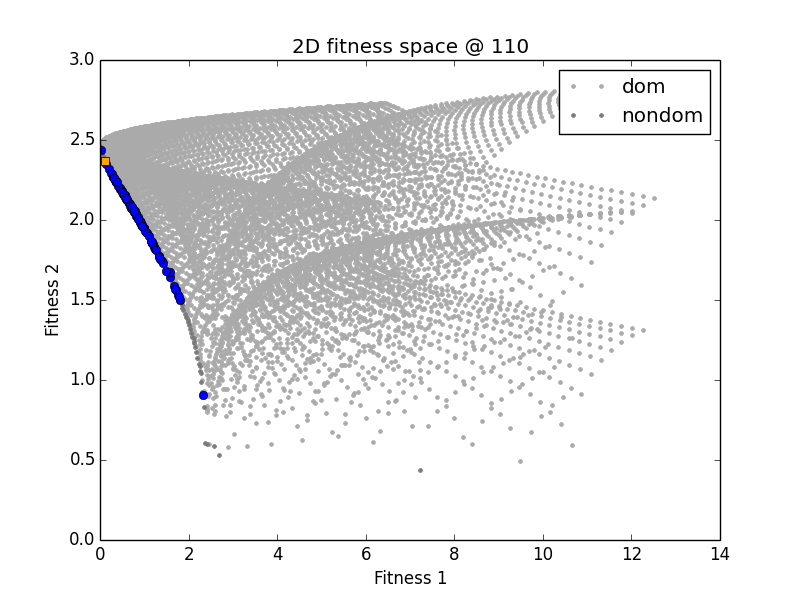
\includegraphics[width=0.45\textwidth]{./images/evaluation_space_perfect_knowledge.png}}      
  \caption{Assume there is good estimation on where the Pareto front locates.}
  \label{fig:perfect_est} %% label for entire figure 
\end{figure}


\subsection{Modifying PSO for multi-objective optimization}

Formally, we give the particle swarm optimization algorithm on multi-objective optimization, which is a modification of Definition \ref{def:pso}.

\begin{enumerate}
\item Scattering particles $ \vec{x}_{i}(0) $ in decision space stochastically
\item Updating whether a particle is non-dominated 
\item Calculating fitness for each particle using equation \eqref{eq:maximin_fitness}
\item Broadcasting the particle with biggest fitness as global best
\item Randomly selecting one from non-dominated particles $ \hat{P^{*}_{S}} $ as personal best for each particle
\item Each particle update its location over time by equations \eqref{eq:up_vel} and \eqref{eq:up_pos}
\end{enumerate}

\section{Stagnation analysis}

A lot of works on analyzing the convergence of the PSO algorithm focus on the stagnation stage.

%\cite{chuan2007standard} considers only the one-order moment, so there uniform stochastic variables are converted into constant. At the same time, ``global best'' and ``personal best" are converted into constant factors. Independent of how fitness function is defined, the problem analysis becomes linear system analysis problem.

\cite{trelea2003particle} and \cite{clerc2002particle} both model the dynamic of the particles as a linear system. 
When the swarm is in stagnation stage, the personal best and the global best becomes stable. 
Let the random parameter be constant, analysis on stability were taken.
\cite{poli2008dynamics} focuses on PSO's sampling distribution and try to explain how it changes over time during stagnation using moment analysis.
By modeling the PSO as a closed-loop system, \cite{samal2007closed} analyze the stability and dynamics on the PSO and extended this analysis to the multi-objective optimization problem [\cite{chakraborty2011convergence}].
By looking at the behavior of a single particle with other particle converged, \cite{schmitt2013particle} analyzed the dynamics of the convergence of a particle and showed the convergence to local optima.

\subsection{Convergence of the swarm}

In approximating the Parteo front, we are interested with that whether the swarm converge into the Pareto set.

We define the stagnation of the swarm in a multi-objective optimization problem as
\begin{itemize}
\item all the particles are non-dominated;
\item the global best is not changed.
\end{itemize}

Define 
\begin{equation}
\label{eq:avg_pos}
\vec{x}(t) = \sum_{ i \in \{ 1, \cdots , n \} } \vec{x_{i}}(t),
\end{equation}

\begin{equation}
\label{eq:avg_vel}
\vec{v}(t) = \sum_{ i \in \{ 1, \cdots , n \} } \vec{v_{i}}(t),
\end{equation}

\begin{equation}
\label{eq:avg_gb}
\vec{x}^{G}(t) = \sum_{ i \in \{ 1, \cdots , n \} } \vec{x}^{G}_{i}(t),
\end{equation}
and
\begin{equation}
\label{eq:avg_pb}
\vec{x}^{P}(t) = \sum_{ i \in \{ 1, \cdots , n \} } \vec{x}^{P}_{i}(t).
\end{equation}

We look at the first moment of the states ,which are $ E(\vec{x}(t)) $ and $ E(\vec{x}(t)) $.
Thus, we can have $ u^{P} = E(u^{P}_{i}(t-1)) $ and $ u^{G} = E(u^{G}_{i}(t-1)) $.
By applying equations \eqref{eq:avg_pos} and \eqref{eq:avg_vel} to equations \eqref{eq:up_pos} and \eqref{eq:up_vel}, we have 
\begin{equation}
\hat{E}(\vec{x}(t)) =  \hat{E}(\vec{x}(t-1)) + \hat{E}(\vec{v}(t)),
\end{equation}
and 
\begin{equation}
\begin{aligned}
E(\vec{v}(t)) & = \chi E(\vec{v}(t-1))   - \chi \phi^{P} u^{P} E(\vec{x}(t-1)) + \chi \phi^{P} u^{P} E(\vec{x}^{P}(t)) \\
& - \chi \phi^{G} u^{G} E(\vec{x}(t-1)) + \chi \phi^{G} u^{G} E(\vec{x}^{G}(t)) \\
& = \chi E(\vec{v}(t-1))  + \chi \phi^{P} u^{P} E(\vec{x}^{P}(t)) + \chi \phi^{G} u^{G} E(\vec{x}^{G}(t)) \\
& - \chi (\phi^{G} u^{G} + \phi^{P} u^{P} ) E(\vec{x}(t-1)). 
\end{aligned}
\end{equation}

Because ``personal best'' is randomly selected from the $ \hat{P}^{*}_{S} $.
We write
\begin{equation}
\label{eq:mean_pb}
E (\vec{x}^{P}(t)) = \bar{x}^{P}
\end{equation}

Also in stagnation, we have global best not changed.
We write 
\begin{equation}
\vec{x}^{G}(t) = \vec{x}^{G},
\end{equation}
thus 
\begin{equation}
\label{eq:mean_gb}
E (\vec{x}^{G}(t)) = \vec{x}^{G}. 
\end{equation}

Applying equations \eqref{eq:mean_gb} and \eqref{eq:mean_pb}, we have
\begin{equation}
\begin{aligned}
E(\vec{v}(t)) & = \chi E(\vec{v}(t-1))  + \chi \phi^{P} u^{P} \bar{x}^{P} + \chi \phi^{G} u^{G} \vec{x}^{G} \\
& - \chi (\phi^{G} u^{G} + \phi^{P} u^{P} ) E(\vec{x}(t-1)). 
\end{aligned}
\end{equation}

We can write the linear model 

\begin{equation}
\begin{bmatrix}
E(\vec{v}(t))
\\ 
E(\vec{x}(t))
\end{bmatrix}
=
\begin{bmatrix}
\chi & - \chi (\phi^{G} u^{G} + \phi^{P} u^{P} )
\\ 
1 & 1
\end{bmatrix}
\begin{bmatrix}
E(\vec{v}(t-1))
\\ 
E(\vec{x}(t-1))
\end{bmatrix}
+ 
\begin{bmatrix}
\chi \phi^{G} u^{G} & \chi \phi^{P} u^{P}
\\ 
0 & 0
\end{bmatrix}
\begin{bmatrix}
\vec{x}^{G}
\\ 
\bar{x}^{P}
\end{bmatrix}.
\end{equation}


\section{Non-stagnation dynamics}

\bibliographystyle{apalike}
\bibliography{reference}

\end{document}
